%------------------------------------------------------------------------
%Editar Diplomado
\hypertarget{cv:modificarColaborador}{\section{Modificar Colaborador}} \label{sec:modificarColaborador}

	Esta funcionalidad le permitirá modificar la información de un colaborador previamente registrado con el fin de corregir o actualizar datos del mismo. 

		\subsection{Procedimiento}

			%Pasos de procedimiento
			\begin{enumerate}
	
			\item Oprima el botón \IUEditar{} de algún registro existente de la pantalla \ref{fig:GestionarColaboradores} ''Gestionar Colaboradores''.
	
			\item Se mostrará la pantalla \ref{fig:modificarColaborador} ''Modificar Colaborador''.
			
			%Pantalla
			\begin{figure}[htbp!]
				\begin{center}
					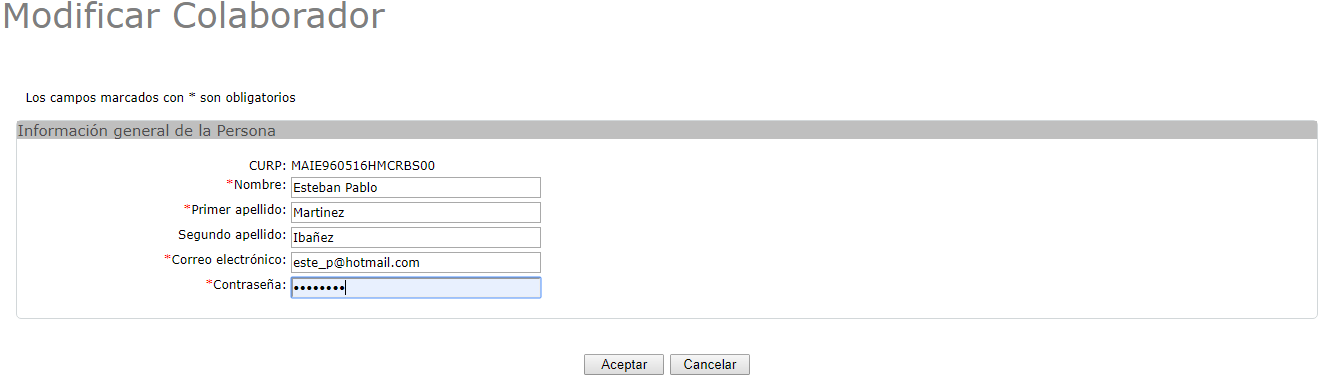
\includegraphics[scale=0.6]{roles/administrador/colaboradores/gestionarColaboradores/pantallas/IU3-2modificarPersona}
					\caption{Modificar Colaborador}
					\label{fig:modificarColaborador}
				\end{center}
			\end{figure}
		
			\item Modifique los datos solicitados por la pantalla.
						
			\item Oprima el botón \IUAceptar.
			
			\item Se mostrará el mensaje \ref{fig:colaboradorEditado} en la pantalla \ref{fig:GestionarColaboradores} ''Gestionar Colaboradores''.
			
			\begin{figure}[htbp!]
				\begin{center}
					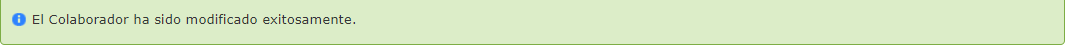
\includegraphics[scale=0.6]{roles/administrador/colaboradores/gestionarColaboradores/pantallas/IU3-2MSG1}
					\caption{MSG: Colaborador Actualizado}
					\label{fig:colaboradorEditado}
				\end{center}
			\end{figure}
			\end{enumerate}